\section{Aufgabe 1}
\subsection{Aufgabe 1 a)}
Die initiale Spotbreite des Protonenstrahls bestimmt sich aus der \enquote{FWHM} größe, die durch python Methoden abgelesen werden kann.
Hierfür wurde eine Maske erstellt mit einer Epsilonumgebung von $0.01$ und
\begin{verbatim}
    eps = 0.01
    mask1 = np.asarray(task1[:,3] > 0.5-eps)
    mask2 = np.asarray(task1[:,3] < 0.5+eps).
\end{verbatim}
Die gefunden boolean Werte werden anschließend auf den gegeben Array angewandt wobei die Resultate bei $-1.05$ und $1.0$ eine Spotbreite von \SI{2.05}{\cm} geben.
\begin{figure}
    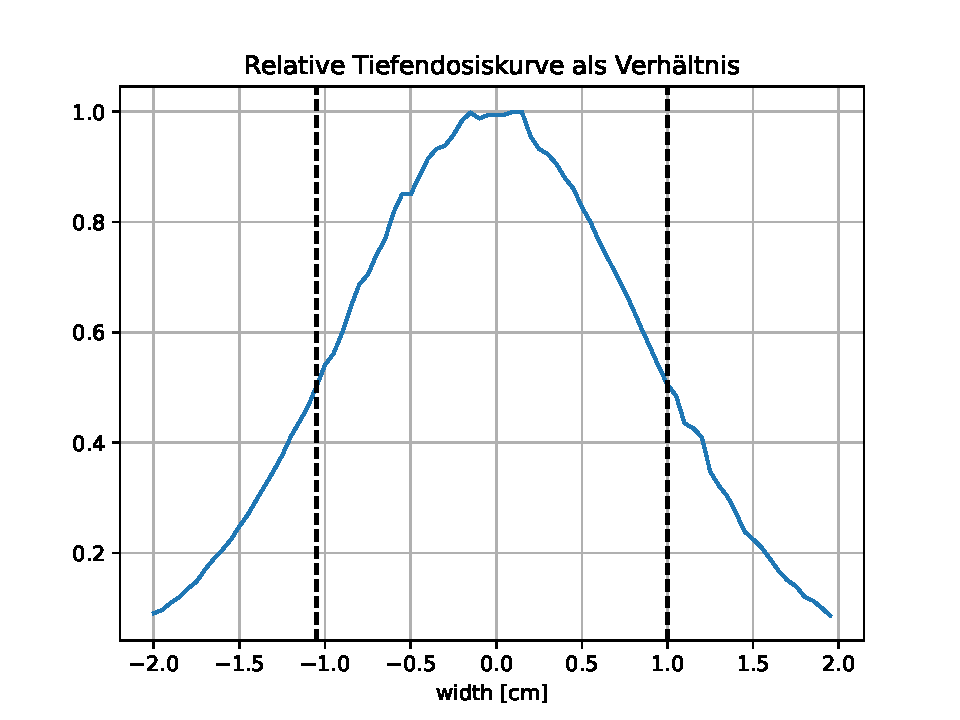
\includegraphics[width = 0.8\textwidth]{../poject/task1/task1a.pdf}
\end{figure}
\noindent
\subsection{Aufgabe 1 b)}
Um die Energien zu bestimmen wird als maßgebliche Kenngröße der $R_{80}$ genommen, die Reichweite der Protonen 
im Medium bei einer Dosis von $80\%$ der maximal Dosis. Gegeben der Datensätze sind die genauen werte bei $0.8 D_{max}$ nicht aufgeführt wodurch zwischen den 
vorhandenen Werten interpoliert werden muss. Hierzu werden zwischen je zwei Werten jeweils 150 leere Zeilen, \enquote{NaN} Einträge eingfügt und diese anschlißend mit einer 
\enquote{pandas} Methode interpoliert. Eine Maske
\begin{verbatim}
    mask1 = np.asarray(df[i][:,3]/np.max(df[i][:,3]) > 0.8-eps)
\end{verbatim}
werden alle werte über 0.8, in einer Epsilonumgebung, gefiltert und der zuletzt gefundene Wert ausgegeben. 

\begin{figure}
    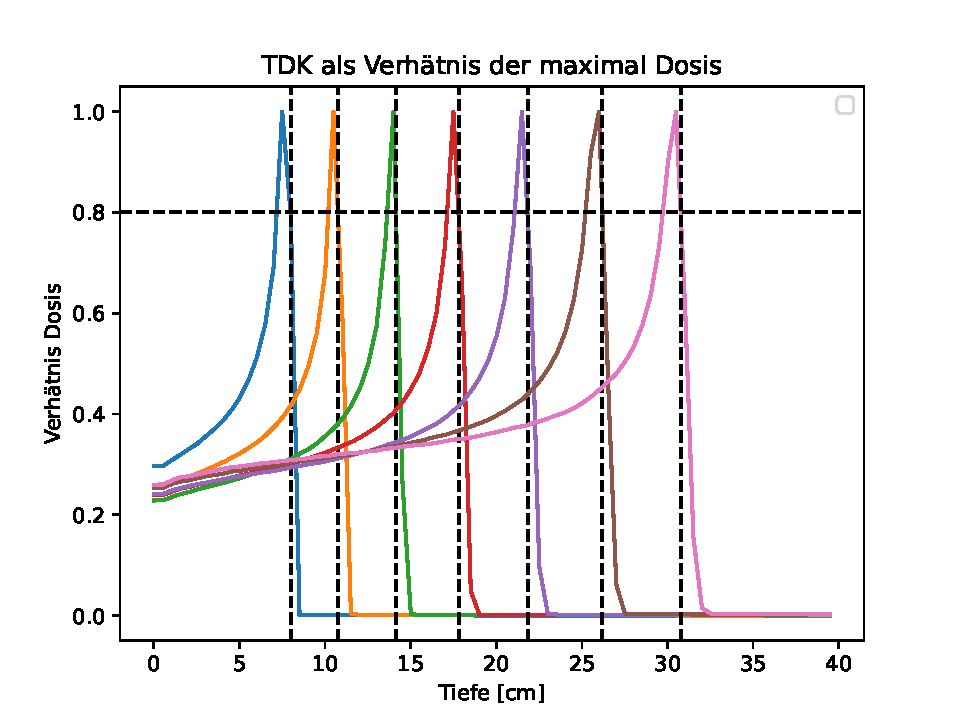
\includegraphics[width = 0.8\textwidth]{../poject/task1/task1b.pdf}
\end{figure} 
\noindent
Mit dem Zusammenhang 
\begin{equation}
    \sigma \approx 0.012 \left( \frac{R_0}{cm} \right) ^{0.935}
\end{equation}
findet sich so ein Fehler auf die Reichweite mit der dann wiederum durch 
\begin{equation}
    E = \left( \frac{R_0}{0.0022} \right)^{1/1.77}
\end{equation}
Die Energien, mitsamt Breite, berechnet werden können.  
Alle Resultate mitsamt Energiebreiten sind dem Appendix zu entenehmen \ref{app}.
\newpage